%! TeX root: ../mpolytope.tex

\begin{frame}
\frametitle{Agenda} \textbf{Plan for today:} 
\begin{itemize}
	\item Quick review of linear programming \& polytopes
	\item Fundamentals of matching theory
	\item The perfect matching polytope
		\begin{itemize}
			\item Bipartite graphs
			\item General graphs
			\item Cubic graphs
		\end{itemize}
\end{itemize}
\end{frame}

\begin{frame}
\begin{center}
	\Large \textbf{Linear Programming \& Polytopes}
\end{center}
\end{frame}

\begin{frame}
\frametitle{Linear Programming}
The goal of \textbf{linear programming} is to maximize (or minimize) a linear objective function subject to a collection of linear constraints. \\
\vspace{0.3cm}
For example:
\begin{align*}
\text{maximize} \quad &z = 5x_1 + 3x_2 - 7x_3 \\
\text{subject to} \quad & x_1 + x_2 + x_3 \leq 12 \\
& 4x_1 + 5x_3 \leq 50 \\
& x_1, x_2, x_3 \geq 0
\end{align*}
\end{frame}

\begin{frame}
\frametitle{Linear Programming}
The goal of \textbf{linear programming} is to maximize (or minimize) a linear objective function subject to a collection of linear constraints. \\
\vspace{0.3cm}

We can express this compactly using matrices:
\begin{itemize}
	\item Goal: Find a vector \( x \) such that \( c^{T} x \) is maximized and \( x \) satisfies the constraints \( A x \leq b \) and \( x \geq 0 \).
	\item (\( x, c \in \mathbb{R}^{n}  \), \( A \in \mathbb{R}^{m \times n} \), and \( b \in \mathbb{R}^{m}  \))
\end{itemize}
\end{frame}

\begin{frame}
    \frametitle{The Dual of an LP}

    Given a linear program in standard form:
    \begin{align*}
        \text{maximize} \quad & c^T x \\
        \text{subject to} \quad & Ax \leq b \\
                                & x \geq 0.
    \end{align*}

    The dual LP is formulated as:
    \begin{align*}
        \text{minimize} \quad & b^T y \\
        \text{subject to} \quad & A^T y \geq c \\
                                & y \geq 0.
    \end{align*}
\end{frame}

\begin{frame}
\frametitle{The Dual of an LP}
The primal and dual LPs provide bounds on each other’s optimal values. If an LP has an optimum at \(x = \hat{x}  \), then its dual also has this optimum (Strong duality theorem).
\end{frame}

\begin{frame}
\frametitle{Polytopes}
A \textbf{polytope} is the convex hull of a finite collection of vectors.
\end{frame}

\begin{frame}
\frametitle{Polytopes}
\begin{figure}
        \centering
        \begin{minipage}{0.32\textwidth}
            \centering
            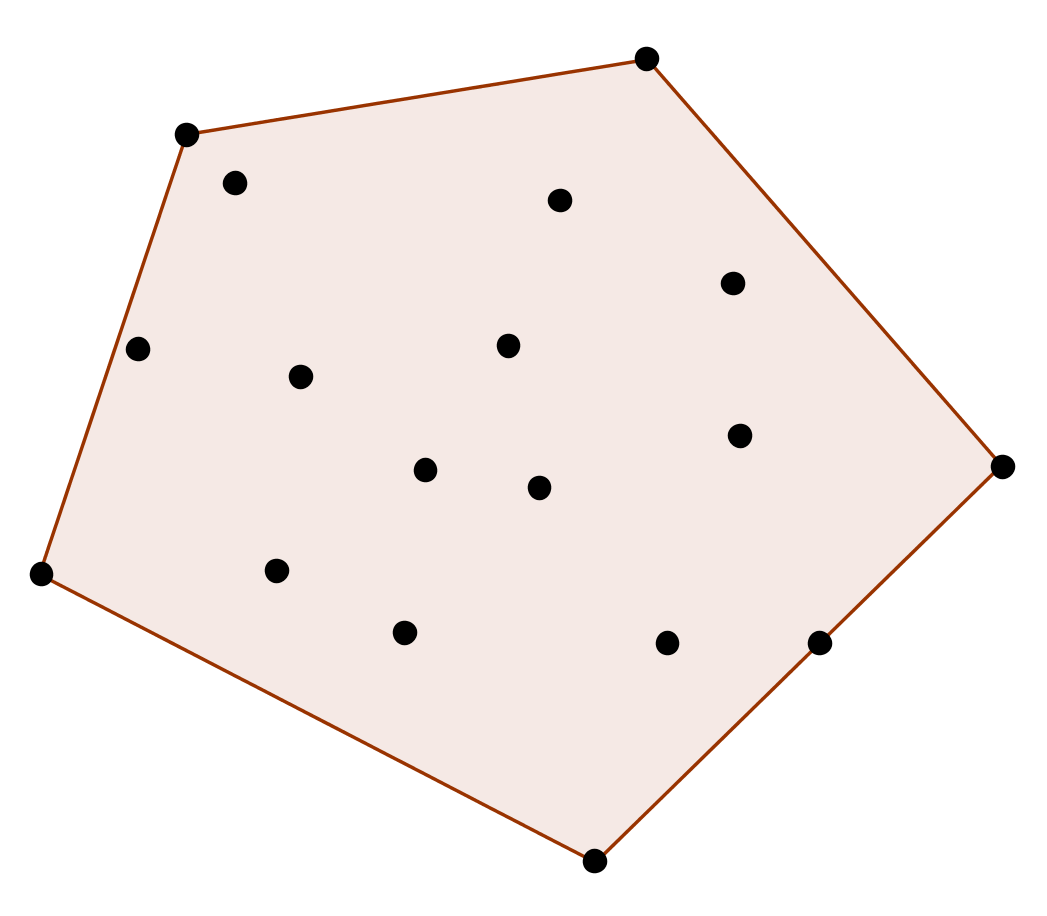
\includegraphics[width=\linewidth]{/Users/jakeg/Desktop/Matching Polytope/images/convexhull.png}
        \end{minipage}\hfill
        \begin{minipage}{0.32\textwidth}
            \centering
            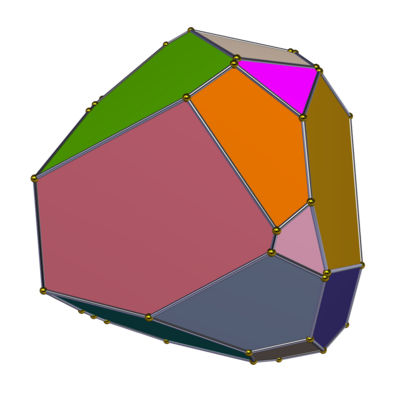
\includegraphics[width=\linewidth]{/Users/jakeg/Desktop/Matching Polytope/images/convex-polytope.png}
        \end{minipage}\hfill
        \begin{minipage}{0.32\textwidth}
            \centering
            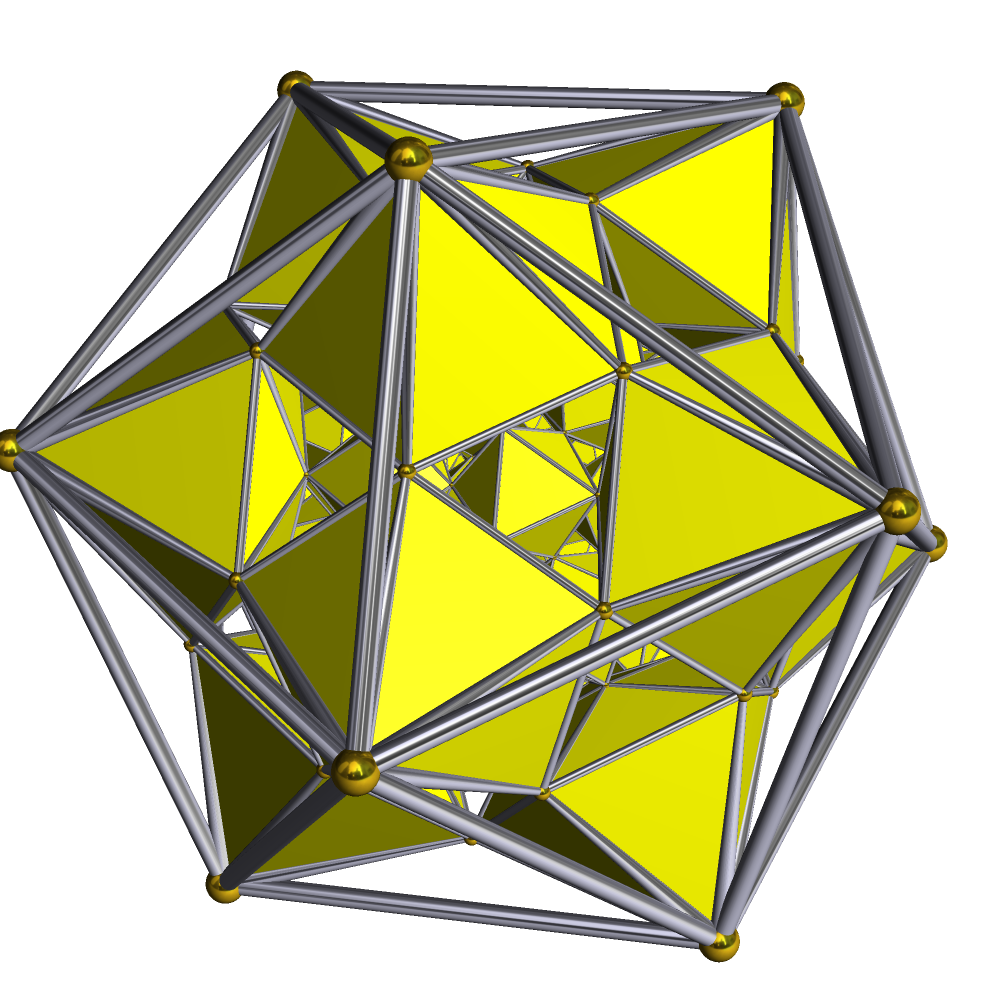
\includegraphics[width=\linewidth]{/Users/jakeg/Desktop/Matching Polytope/images/600cell.png}
        \end{minipage}
\end{figure}
\end{frame}

\begin{frame}
\begin{center}
\Large How are polytopes related to LP?
\end{center}
\end{frame}

\begin{frame}
\begin{center}
	{\Large How are polytopes related to LP?} \\
	\vspace{0.3cm}
	\emph{via an equivalent definition...} 
\end{center}
\end{frame}

\begin{frame}
\frametitle{Polytopes \& LP}
A vector \( \mathbf{x} \) is called a \textbf{feasible solution} if it satisfies the linear constraints of the LP, i.e. if \( A \mathbf{x} \leq \mathbf{b} \) and \( \mathbf{x} \geq \mathbf{0} \).\\

\vspace{0.3cm} The set \( P = \{ \mathbf{x} \geq \mathbf{0} : A\mathbf{x} \leq \mathbf{b} \}  \) of all feasible solutions is called a \textbf{polyhedron}. 
\begin{itemize}
	\item Bounded polyhedra are called \textbf{polytopes}.
	\item If the set of all feasible solutions to an LP is a polytope, then one of its corners is an optimum.
\end{itemize}
\end{frame}

\begin{frame}
\frametitle{The Big Picture}
We would like to solve combinatorial optimization problems using algorithms.\\

\vspace{0.3cm}
Some examples:
\begin{itemize}
	\item Finding min-weight edge or vertex covers in graphs.
	\item Finding (pure, mixed, correlated) Nash equilibria in games.
	\item Finding max flows and min cuts in flow networks.
	\item Finding min-weight perfect matchings in graphs.
\end{itemize}
\vspace{0.3cm}
If we can reduce these problems to solving linear programs, we can leverage efficient LP solvers to obtain optimal solutions.
\end{frame}

\begin{frame}
\begin{center}
\Large This talk is about the connection between linear programming, polytopes, and perfect matchings.
\end{center}
\end{frame}

\begin{frame}
\frametitle{Perfect Matchings}
A \textbf{matching} in a simple graph \( G = (V,E) \) is a subset \( M \subseteq E \) of edges such that no two edges in \( M \) share an end. So every vertex \( v \in V \) is incident to \emph{at most} one edge in \( M \). \\

\vspace{0.3cm}

A matching \( M \) is \textbf{perfect} if every vertex \( v \in V \) is incident to \emph{exactly} one edge in \( M \). 
\end{frame}

\begin{frame}
\frametitle{Perfect Matchings}
A perfect matching (red edges) in the Petersen graph:
\begin{center}
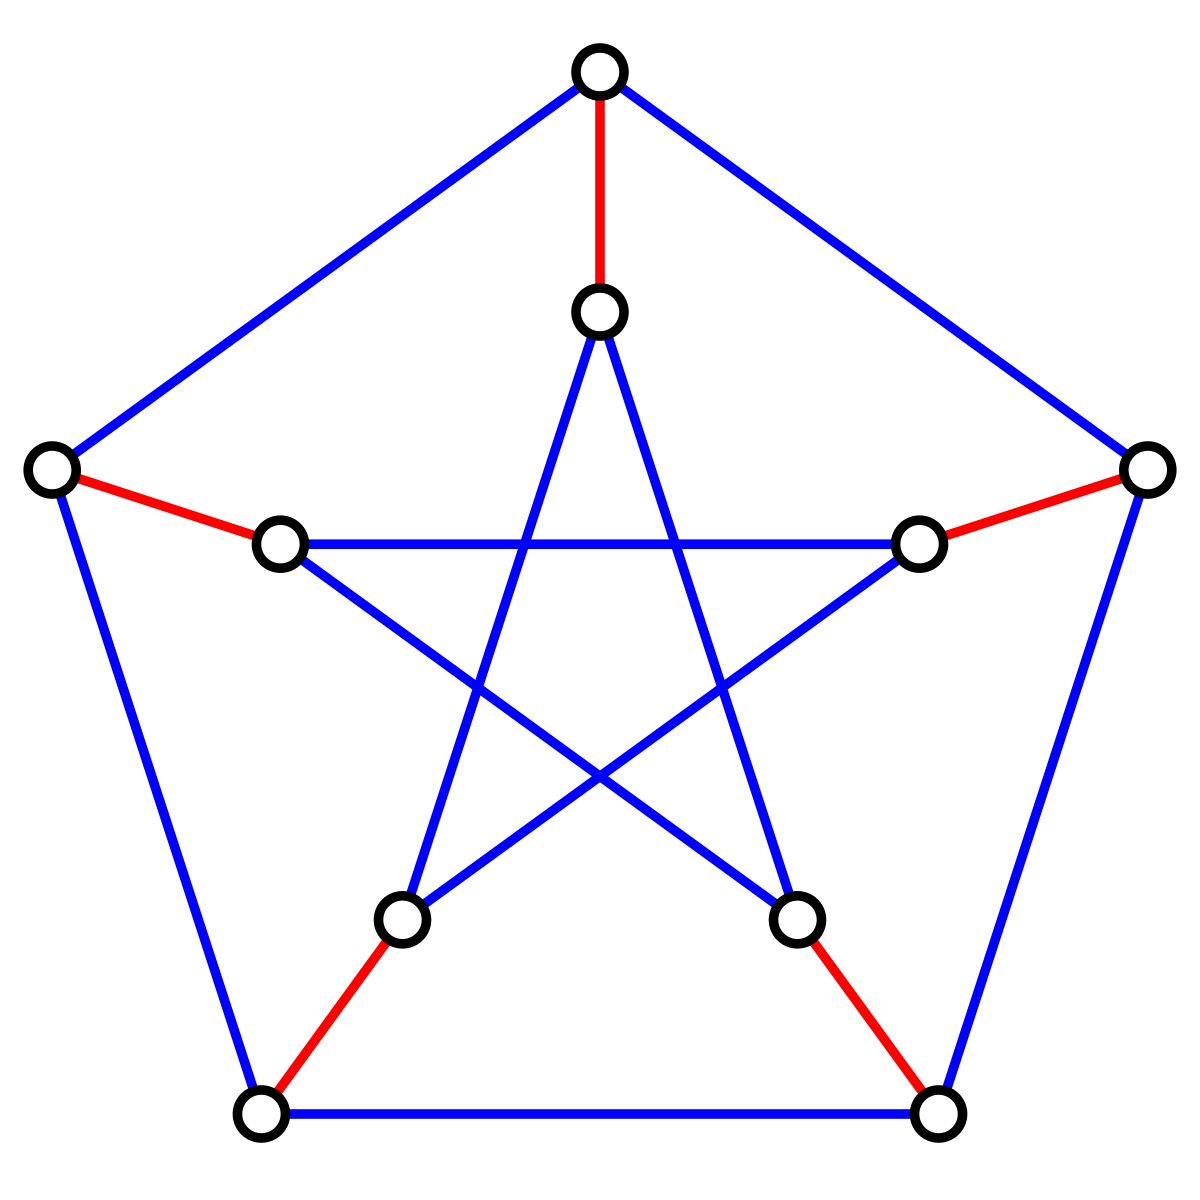
\includegraphics[scale=0.1]{/Users/jakeg/Desktop/Matching Polytope/images/peter-match.png}
\end{center}
\end{frame}
